\documentclass{article}
\usepackage{enumitem}
\usepackage{titlesec}
\usepackage{titling}
\usepackage[margin=1in]{geometry}
\usepackage{underscore}
\usepackage{graphicx}
\graphicspath{{./resources/}{IR}}
\usepackage{fancyhdr}
\pagestyle{fancy}
\fancyhead{}
\lhead{}
\chead{Austen Nelson --- Zhengmao Zhang --- Xiaoran Ge --- Xingjian Wang --- Michael Kay --- Thomas Pollard}
\rhead{}

\renewcommand{\maketitle}{
   \begin{center}
      {\Huge \bfseries Design Document}
   \end{center}
}

\newlist{steps}{enumerate}{1}
\setlist[steps, 1]{label = \underline{\hspace{2em}} Step \arabic*:}

\setlength{\parindent}{0em}

\begin{document}

\maketitle
\tableofcontents
\pagebreak

\section{Introduction}
This design document mainly introduces the system and software design of this project. After analyzing all the requirements of this project, our team set out to establish the overall architecture of the entire system based on the requirements. After discussions between the teams, we chose this structure and added enough details in this design document  to have a reference basis in the future development process.This design document can effectively improve the development efficiency of the team and ensure the feasibility and integrity of the final product.

\subsection{Purpose and Scope}
The purpose of this design document is to explain the design of the entire system in detail so that developers can understand the business logic of each part of the system, and to check the correctness of the development process at any time during the development process. The contents of this design document include the design of the entire system, details of each part of the system, and the relationship between each part of the system.

This document serves as the basis for the data management system required by the ChocoAn organization. You can read this document to understand the basic functions of the entire data management system and how our team implements them. This data management system meets the management needs of the ChocAn organization by collecting the data of each member, and does some actions like  adding, reducing, deleting, searching the data.

\subsection{Target Audience}
This design document is applicable to all developers of this project and maintenance personnel who need to maintain the system in the future. After reading this document, anyone can have a clear understanding of the entire project and be able to make some changes and maintenance to the project.

\subsection{Terms and Definitions}
\begin{itemize}
   \item ChocAn --- Chocoholics Anonymous. 
   \item OOP --- Object Oriented Programming.
   \item Functional Requirements --- A Functional Requirement (FR) is a description of the service that the software must offer.
   \item Software Design Patterns --- Software design pattern is a general, reusable solution to a commonly occurring problem within a given context in software design.
   \item UI --- User Interface.
   \item API --- Application Programming Interface.
   \item Client/Server model --- For the usage of this document “Client” will refer to requests from outside of this software and “Server” will refer to internal operation. Client software includes but is not limited to UI, EFT, accounting, and communications.
\end{itemize}

\section{Design Considerations}
This section details the choices about the design of the software. Constraints and dependencies investigates limitations and requirements of the software. Methodology explains the general design approach and programming paradigms used to develop the software.

\subsection{Constraints and Dependencies}
What constrains, either functional or non-functional were you required to adhere to in designing and implementing your system?
Concurrency Control - This system will be accessed and modified by different groups simultaneously. In order to maintain data coherency, concurrency protection is practiced whenever writing to disk.
Data formatting - Data is recorded and reported in a consistent manner across all modules of the software. 

\subsection{Methodology}
To implement the ChocAn data system the Object Oriented Programming (OOP) paradigm is employed. This is a suitable approach for this project as each subsystem will require components that can be represented as loosely coupled objects. OOP concepts such as composition and inheritance will be used to create a safe and functional type system that guides the structure of the software. Discrete top level systems will be broken into modules usings C++ namespaces to provide safety and program segmentation. This will facilitate evolution and maintenance of the product.

\section{System Overview}
The data processing system will be divided into three primary modules. Each of these modules are for the different modes that the software provides. These modes are provider, manager, and interactive.

  \begin{figure}[h!]
	\centering
	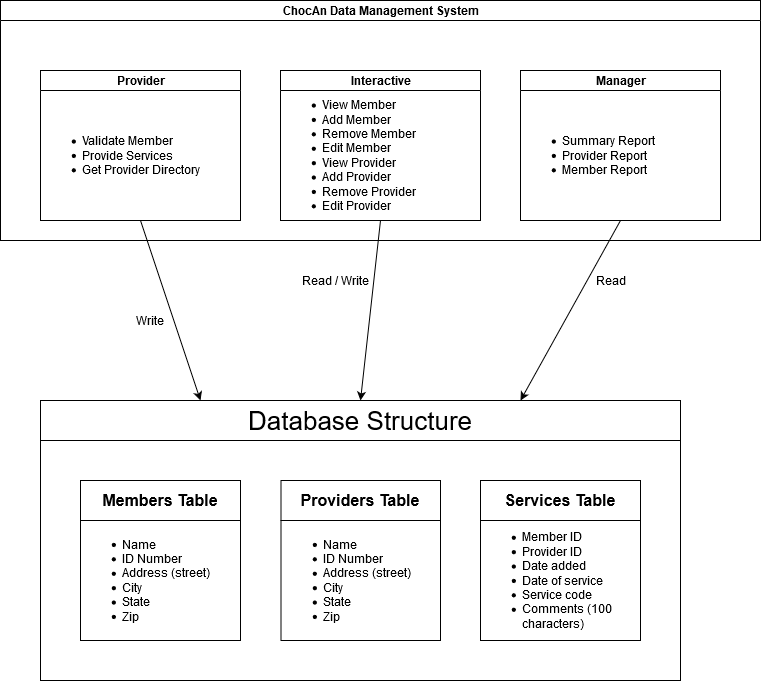
\includegraphics[width=0.8\linewidth]{SystemOverview.png}
	\caption[System Overview]{System Overview}
	\label{fig:P1compileP0-1}
  \end{figure}

Each of these modules will be represented as C++ class objects. The terminal used to simulate the usage of these API’s will ask which mode the user would like to simulate and then provide text based menus to access each of the functionalities.

Data management will be handled with three database tables that will be queried to produce the reports and calculate billing. These tables will be stored as external files on disk in CSV format.

The following objects will be used:
\begin{itemize}
   \item Person --- A base class for Member and Provider
   \item Member --- A member, the members information
   \item Provider --- A provider, the providers information
   \item Service --- An individual service, the service information
   \item ProviderDirectory --- Table to generate services directory to look up service codes
   \item InteractiveModule --- Contains the API to manage database contents (members and providers)
   \item ManagerModule --- Contains the API to run manager reports
   \item ProviderModule --- Contains the API to provide services and request service directory
\end{itemize}

\section{System Architecture}
The system architecture will be split into three modules, the provider, interactive, and manager module. The subsystem includes several objects. Some of these objects will be included in multiple of the software modules. The only objects with client side APIs are the ProviderModule, InteractiveModule, and ManagerModule. The rest of the objects API will be for internal usage only. The following chart shows the relationship between these objects. Dotted lines demonstrate multiple systems use the subsystem.

  \begin{figure}[h!]
	\centering
	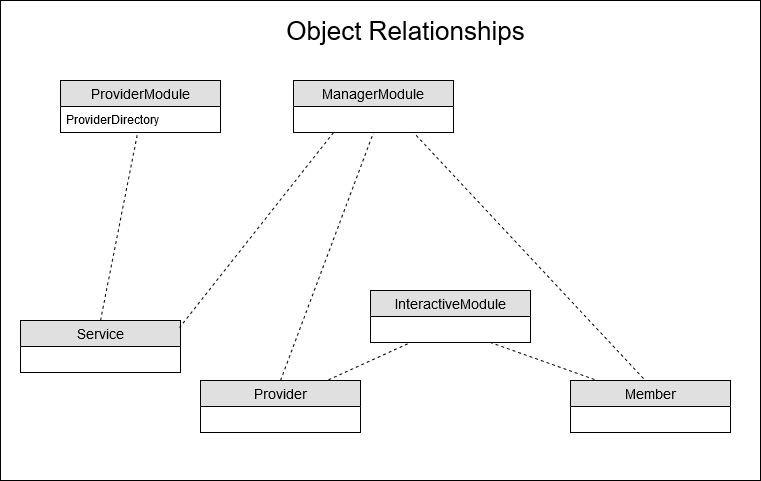
\includegraphics[width=0.8\linewidth]{architecture.png}
	\caption[System Architecture]{System Architecture}
	\label{fig:P1compileP0-1}
  \end{figure}

\subsection{Person}
\subsubsection{Member}
\subsubsection{Provider}
Member and Provider - Derived from Person class

\subsection{Service}
  \begin{figure}[h!]
	\centering
	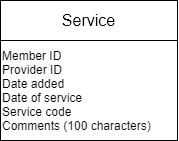
\includegraphics[width=0.3\linewidth]{service.png}
	\caption[Service]{Service}
	\label{fig:P1compileP0-1}
  \end{figure}
Service - An individual service, the service information

\subsection{InteractiveModule}
  \begin{figure}[h!]
	\centering
	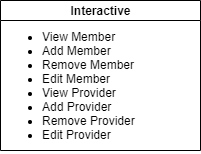
\includegraphics[width=0.3\linewidth]{interactiveModule.png}
	\caption[Interactive Module]{Interactive Module}
	\label{fig:P1compileP0-1}
  \end{figure}
InteractiveModule - Contains the API to manage database contents (members and providers)

\pagebreak
\subsection{ManagerModule}
  \begin{figure}[h!]
	\centering
	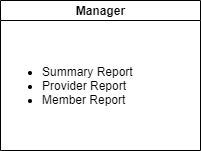
\includegraphics[width=0.3\linewidth]{managerModule.png}
	\caption[Manager Module]{Manager Module}
	\label{fig:P1compileP0-1}
  \end{figure}
ManagerModule- Contains the API to run manager reports

\subsection{ProviderModule}
  \begin{figure}[h!]
	\centering
	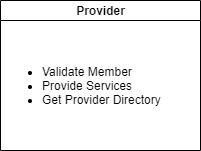
\includegraphics[width=0.3\linewidth]{providerModule.png}
	\caption[Provider Module]{Provider Module}
	\label{fig:P1compileP0-1}
  \end{figure}
ProviderModule - Contains the API to provide services and request service directory
\subsubsection{ProviderDirectory}
  \begin{figure}[h!]
	\centering
	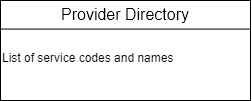
\includegraphics[width=0.3\linewidth]{providerDirectory.png}
	\caption[Provider Directory]{Provider Directory}
	\label{fig:P1compileP0-1}
  \end{figure}
ProviderDirectory - Table to generate services directory to look up service codes.

\section{Detailed System Design}
\subsection{Person}
\textbf{Data structures:}
\begin{itemize}
   \item string name, city, state
   \item uint ID, zip
\end{itemize}
\textbf{Functions:}
\begin{itemize}
   \item string getName()
   \item string getCity()
   \item string getState()
   \item uint getZip()
   \item uint getID()
\end{itemize}
The constructor will require all of the fields up front to verify that the data is valid. The object provides methods to set and get data fields. These setters and getters are used to update and view member data as well as generate reports. Most of the fields will be stored in C++ strings. ID and zip will be stored as unsigned integers. ID’s are 9 digits long so a standard 32 bit unsigned int will be sufficient.

\subsubsection{Member: public Person}
\textbf{structures:}
\begin{itemize}
   \item bool suspended
\end{itemize}
\textbf{Functions:}
\begin{itemize}
   \item Member(string name, uint memberID, string city, string state, uint zip)
\end{itemize}
The Member object is primarily a container for data associated with a ChocAn member. Member status is stored as a bool (true means suspended). 

\subsubsection{Provider: public Person}
The Provider object is a container for data associated with a specific provider. Currently it doesn’t have any data or functionality beyond what is available in Person but it is a seperate class to anticipate possible change to the Provider abstraction in the future.

\subsection{Service}
\textbf{Data Structures:}
\begin{itemize}
   \item uint memberID, providerID, serviceCode
   \item time_t timeOfService, timeRecorded
   \item string comments
\end{itemize}
\textbf{Functions:}
\begin{itemize}
   \item uint getMemberID()
   \item uint getProvderID()
   \item uint getServiceCode()
   \item time_t getTimeOfService()
   \item time_t getTimeRecorded
   \item string getComments()
\end{itemize}
The service object is an abstraction for a service provided by a ChocAn provider to a member. The fields of the service will include the member ID, provider ID, and the service code as unsigned ints. The time of service and time of entry will be saved using the time_t type from the C standard <ctime> header. The functions will provide a way to access this private data. The constructor will require all of the data needed to create the service object.

\subsection{InteractiveModule}
\textbf{Data Structures:}
\begin{itemize}
   \item unordered_map<uint, Member>   //hashmap keyed on ID
   \item unordered_map<uint, Provider>   //hashmap keyed on ID
\end{itemize}
\textbf{Functions:}
\begin{itemize}
   \item int init()
   \item int displayMember(uint memberID)
   \item int addMember()
   \item int removeMember(unit memberID)
   \item int editMember(uint memberID)
   \item int displayProvider(uint memberID)
   \item int addProvider()
   \item int removeProvider()
   \item int editProvider(uint memberID)
   \item int writeOut()
\end{itemize}
The InteractiveModule provides an interface for ChocAn data center employees to manage records of members and providers. To start interactive mode the init() function is called from the object. This will display a menu that provides options to add, remove, or edit providers and members or save and exit. When the changes are made the save and exit option is selected and the database is updated with the changes. The members and providers will be stored in an unordered_map (hashmap) C++ data structure. This gives constant time access and insertion to members and providers keyed on ID.

\subsection{ManagerModule}
\textbf{Data Structures:}
\begin{itemize}
   \item map<time_t, Service>  services
   \item unordered_map<uint, Provider> providers
   \item unordered_map<uint, Member> members
\end{itemize}
\textbf{Functions:}
\begin{itemize}
   \item int generateWeeklyReports()
   \item If this fails, errors will be in the <date>.log file
   \item int generateSummaryReport()
   \item string generatePersonReportBase(Person\& person)
   \item int generateProviderReport(uint providerID)
   \item int generateMemberReport(uint memberID)
\end{itemize}
The ManagerModule is where all the reports will be run from. It will provide functions to run reports on specific providers or members as well as running a weekly summary report. The generateWeeklyReports() method will run each Friday and run a report on every member and provider as well as the summary for that week. All the services will be read in from the database into a map C++ standard library data structure keyed on time added. Because map is implemented as a balanced tree, this allows efficient access to any given time frame and preserves order that the services were added to the system. Providers and members are loaded in from the database into the unordered_map so any Person can be retrieved in constant time. The algorithms to generate the reports are as follows:
Provider Report - Find the provider information from the providers map and pass this person object to the base report method to generate a header for the report. Then filter the services tree to only include services from the last week and that are associated with the provider in question.
Member Report - Same a Provider.
Summary Report - Filter the services map to only include services from the last week. Create a local struct called Total with two fields, an int for service count and a float for total billing. Create a local unordered_map<uint, Total> where the key in the provider ID and the value is the running sum of the providers data. This map will be used to keep track of each unique provider encountered. Iterate over the filtered service map and for each service:
get the provider ID
try to find the provider in the unordered_map
if found: dereference the iterator returned and increment the count and add the price for the current service to the totalBilling field in the struct
else: create a new Total struct and set its count variable to one and its totalBilling field to the billing value. Add the key value pair of the providerID and the new Total struct to the unordered_map
    Then iterate over the (key, value) pairs in the unordered_map. For each:
Look up the provider’s name from the key and write it to the file
Write the count and totalBilling variables to the file from the associated key
Weekly Report - Run the Provider Report and Member Report for every provider and member in the unordered_maps. Then run the Summary Report.

\subsection{ProviderModule}
\textbf{Data Structures:}
\begin{itemize}
   \item ProviderDirectory directory
   \item uint providerID
\end{itemize}
\textbf{Functions:}
\begin{itemize}
   \item int init(uint providerID)
   \item int validateMember(uint memberID)
   \item int provideService(Service\& service)
   \item int getProviderDirectory()
\end{itemize}
The ProviderModule provides an API for the providers to verify members and provide services. The init() function will run a simulated menu so these functionalities can be tested. ValidateMember will access the members file and search for a member with a matching ID and check if the Member is suspended or not. provideServices() will take a constructed Service object and then display back the details and ask for confirmation that all the information is correct. If so, it will send the service to the data file. getProviderDirectory() will write all the services with codes to a file called directory.txt.

\subsubsection{ProviderDirectory}
\textbf{Data Structures:}
\begin{itemize}
   \item map<service, uint> services
\end{itemize}
\textbf{Functions:}
\begin{itemize}
   \item int generateDirectory()
\end{itemize}
The ProviderDirectory object will be used to lookup service names and to display the preview when a service is being provided. The map data structure is chosen because the c++ standard library implements maps using a balanced red/black tree. This allows us to sort the services by name as stated in the requirements document and allows code lookup in log(n) time complexity. If the program requires in the future to add to this structure it will also provide insertion at the same time complexity. GenerateDirectory will write the directory to a file called directory.txt.

\end{document}
